\documentclass[11pt]{article}
\usepackage{amsmath}
\usepackage{amssymb}
\usepackage{graphicx}
\usepackage{fancyhdr}
\usepackage{enumerate}
\usepackage{titlesec}
\usepackage[colorlinks=true,urlcolor=blue]{hyperref}

\titlespacing{\subsubsection}{0pt}{0pt}{0pt}

% No page numbers
%\pagenumbering{gobble}
\newenvironment{code}{\fontfamily{pcr}\selectfont} {\par}

% MARGINS (DO NOT EDIT) ---------------------------------------------
\oddsidemargin  0.25in \evensidemargin 0.25in \topmargin -0.5in
\headheight 0.2in \headsep 0.1in
\textwidth  6.5in \textheight 9in
\parskip 1.25ex  \parindent 0ex \footskip 20pt
% ---------------------------------------------------------------------------------

% HEADER (DO NOT EDIT) -----------------------------------------------
\newcommand{\problemnumber}{0}
\newcommand{\myname}{name}
\newfont{\myfont}{cmssbx10 scaled 1000}
\pagestyle{fancy}
\fancyhead[L]{\myfont Question \problemnumber, Problem Set 1, CS229}
\fancyhead[R]{John Mern, jmern91@stanford.edu}
\newcommand{\newquestion}[1]{
\clearpage % page break and flush floats
\renewcommand{\problemnumber}{#1} % set problem number for header
\phantom{}  % Put something on the page so it shows
}
% ---------------------------------------------------------------------------------


% BEGIN HOMEWORK HERE
\begin{document}

% Question 1
\newquestion{1(a)}
The algorithm converged in about 30,0000 iterations for dataset A, however, it did not converge in over 3M iterations for set B. 

\newquestion{1(b)}

As can be seen below, the gradient of A quickly converges to it's asymptotic limit of zero. The gradient for B, however, remains non-zero as the gradient decay rate flattens. 

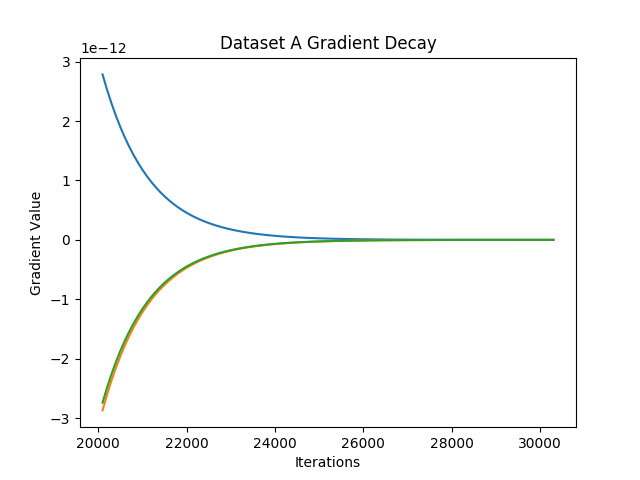
\includegraphics[scale=0.4]{P1b_1.png}
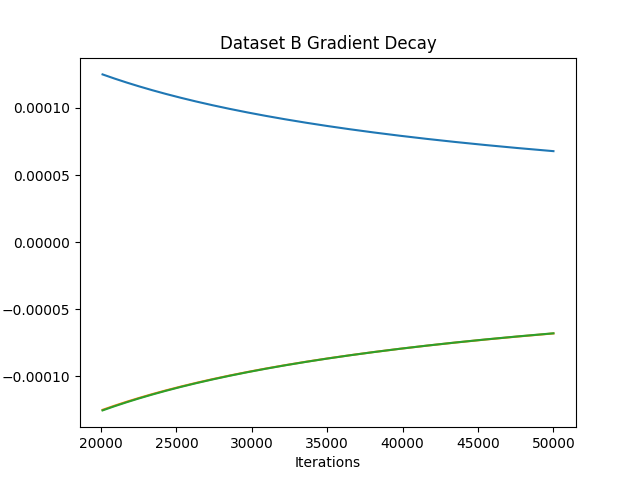
\includegraphics[scale=0.4]{P1b_2.png}

This is likely due to the fact that, while dataset A has no clear margin between the positive and negative examples, dataset B is almost perfectly separable. For a set that is nearly perfectly separable, the gradient becomes exteremely small for values near the optimal solution. As we can see in the expression for the gradient of log-likelihood $ (y - h_{\theta}(x))x_j$ with $h_\theta(x) = \frac{1}{1 + e^{-\theta^Tx}}$, for correctly categorized values, increasing theta will always increase the log-likelihood. This will cause the gradient to decay very slowly, as theta can alwasy be increased to improve performance. 

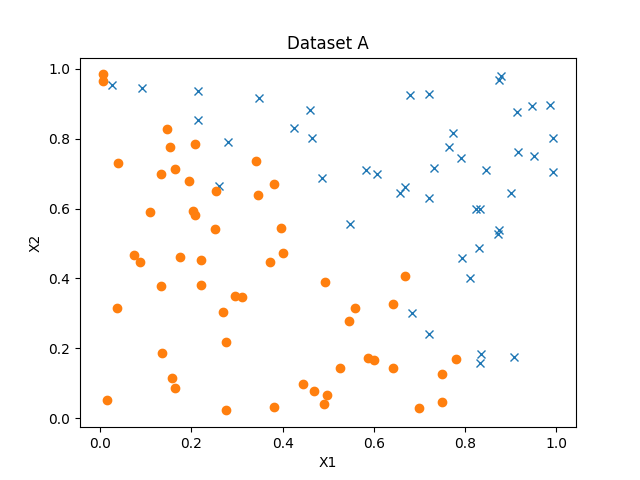
\includegraphics[scale=0.4]{P1b_3.png}
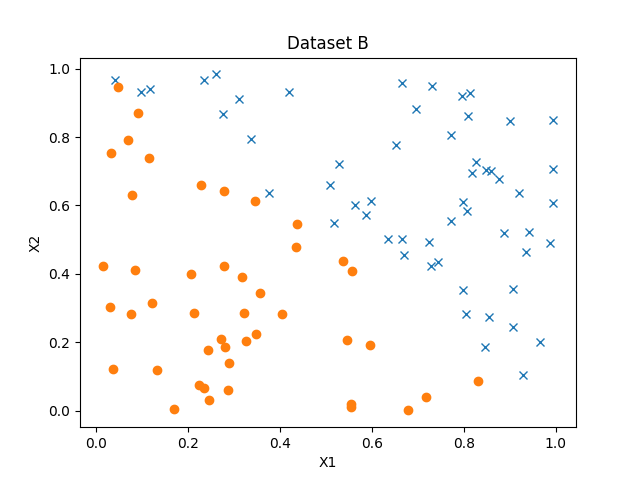
\includegraphics[scale=0.4]{P1b_4.png}

By removing the points that cause the non-zero margin in A, we get the resulting dataset shown below. Running the regression on this does not converge after 500K iterations. 

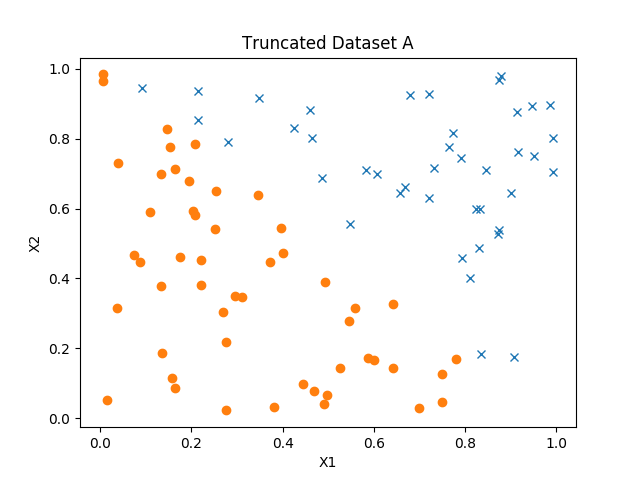
\includegraphics[scale=0.4]{P1b_5.png}

\newquestion{1(c)}

i. This will not aid significantly in convergence of separable sets. The gradient signal will still approach zero asymptotically as in B, and changing the learning rate will not change this trend. 

ii. This will allow the algorithm to satisfy the convergence condition. By decreasing the learning rate significantly quickly, the update on theta can be made to go toward zero, satisfying the convergence condition. This may cause the iterations to end prematurely however, as the gradient may still be large. 

iii. This should aid in convergence. L2 regularization causes weights to tend toward small values, offsetting the trend motivating the theta to always increase for separable sets. 

iv. This would not help. The features are already of similar dimension.

v. This should help by causing more points to cross the optimal hyperplane, increasing the strength of the gradient signal.  

\newquestion{1(d)}

SVMs seek to maximize the margin between the separating hyperplane and the supporting hyperplane of each set. If using a hinge-loss with fixed margin, perfectly separable cases can be handled well. 

\newquestion{1 (code)}

\begin{code}
\begin{verbatim}
import numpy as np 
import matplotlib.pyplot as plt

from lr_debug import * 

import pdb



def logistic_regression(X, Y, ints):
    m, n = X.shape
    theta = np.zeros(n)
    learning_rate = 10

    i = 0
    I = []
    Grad = []
    while True:
        i += 1
        prev_theta = theta
        grad = calc_grad(X, Y, theta)
        theta = theta  - learning_rate * (grad)
        if i % 100 == 0:
        	Grad.append(grad)
        	I.append(i)
        if i % 10000 == 0:
            print('Finished %d iterations' % i)
        if np.linalg.norm(prev_theta - theta) < 1e-15:
            print('Converged in %d iterations' % i)
            break
        if i >= ints:
        	print('Did not converge')
        	break
    return Grad, I

Xa, Ya = load_data('data_a.txt')
Xb, Yb = load_data('data_b.txt')

Xa_p = Xa[Ya>0, :]
Xa_n = Xa[Ya<0, :]

Xb_p = Xb[Yb>0, :]
Xb_n = Xb[Yb<0, :] 

gradA, IA = logistic_regression(Xa, Ya, 50000)

gradB, IB = logistic_regression(Xb, Yb, 50000)

gradA = np.array(gradA)
plt.figure()
plt.plot(IA[200:], gradA[200:,0])
plt.plot(IA[200:], gradA[200:,1])
plt.plot(IA[200:], gradA[200:,2])
plt.title('Dataset A Gradient Decay')
plt.xlabel('Iterations')
plt.ylabel('Gradient Value')
plt.show()

gradB = np.array(gradB)
plt.figure()
plt.plot(IB[200:], gradB[200:,0])
plt.plot(IB[200:], gradB[200:,1])
plt.plot(IB[200:], gradB[200:,2])
plt.title('Dataset B Gradient Decay')
plt.xlabel('Iterations')
plt.ylabel('Gradient Value')
plt.show()

plt.figure()
plt.plot(Xa_p[:,1], Xa_p[:,2], 'x')
plt.plot(Xa_n[:,1], Xa_n[:,2], 'o')
plt.title('Dataset A')
plt.xlabel('X1')
plt.ylabel('X2')
plt.show()

plt.figure()
plt.plot(Xb_p[:,1], Xb_p[:,2], 'x')
plt.plot(Xb_n[:,1], Xb_n[:,2], 'o')
plt.title('Dataset B')
plt.xlabel('X1')
plt.ylabel('X2')
plt.show()

Xap_ = []
Yap_ = []

for i in range(Xa_p.shape[0]):
	if 1 - Xa_p[i,1] <= Xa_p[i,2]:
		Xap_.append(Xa_p[i,:])
		Yap_.append(1)

Xap_ = np.array(Xap_)
Yap_ = np.array(Yap_)

Xan_ = []
Yan_ = []

for i in range(Xa_n.shape[0]):
	if 1 - Xa_n[i,1] >= Xa_n[i,2]:
		Xan_.append(Xa_n[i,:])
		Yan_.append(-1)

Xan_ = np.array(Xan_)
Yan_ = np.array(Yan_)
plt.figure()
plt.plot(Xap_[:,1], Xap_[:,2], 'x')
plt.plot(Xan_[:,1], Xan_[:,2], 'o')
plt.title('Truncated Dataset A')
plt.xlabel('X1')
plt.ylabel('X2')
plt.show()

Xa_ = np.vstack([Xap_, Xan_])
Ya_ = np.vstack([Yap_.reshape([-1,1]), Yan_.reshape([-1,1])]).squeeze()
grad_, I_ = logistic_regression(Xa_, Ya_, 500000)
\end{verbatim}
\end{code}

\newquestion{2(a)}

Starting from the definition of log-likelihood of logistic regression, 

$$ \nabla_\theta l_\theta = \sum_{i=1}^m(\frac{y^i}{g(\theta^Tx^i)} - \frac{1 - y^i}{1 - g(\theta^Tx^i)})\nabla_\theta g(\theta^T x^i) $$

$$ \nabla_\theta g(\theta^T x^i) = g(\theta^T x^i)(1 - g(\theta^T x^i))x^i $$ 

Substituting this back in and simplifying, 

$$ \nabla_\theta l_\theta = \sum_{i=1}^m(y^i - g(\theta^Tx^i))x^i $$ 

For the optimal $\theta$, this equals zero, giving the following. 

$$ \sum_{i=1}^m y^i x^i = \sum_{i=1}^m g(\theta^Tx^i)x^i $$ 

This equality needs to hold for all dimensions of $x$, including the bias. The equality in this dimension yields, 

$$ \sum_{i=1}^m y_0^i = \sum_{i=1}^m g(\theta^Tx^i) = \sum_{i=1}^m h_\theta(x) $$

$$ \sum_{i=1}^m \textbf{1} \{y^i = 1\} = \sum_{i=1}^m h_\theta(x) $$ 

$$ \frac{\sum_{i=1}^m \textbf{1} \{y^i = 1\}}{|i\in I_{0,1}|} = \frac{\sum_{i=1}^m h_\theta(x)}{|i\in I_{0,1}|} $$

\newquestion{2(b)}

A perfectly calibrated model will not necessarily achieve perfect accuracy. Consider $y \in {1,1,-1,-1} $, and $ h_\theta (x) = 0.5 $

$$ \frac{\sum_{i=1}^m h_\theta(x)}{m} = 0.5 = \frac{\sum_{i=1}^m \textbf{1} \{y^i = 1\}}{m} $$

This model is perfectly calibrated, however, it will not be perfeclty accurate as the hypothesis is simply a random guess. 

A model that is perfectly accurate on any test set will necessarilly be perfectly calibrated. For $y^i =1, h_\theta(x^i) = 1 $, and for $y^i =0, h_\theta(x^i) = 0$.

\newquestion{2(c)} 

A model with L2 regularization cannot be perfectly calibrated. The gradient term for such a loss term is shown below. 

$$ \nabla_\theta l(\theta) + \nabla_\theta L2 $$

$$ \nabla_\theta L2 = 2\theta $$ 

Starting at the end of part a, we see 

$$ \sum_{i=1}^m y^i x^i = \sum_{i=1}^m g(\theta^Tx^i)x^i + 2 \theta $$

$$ \sum_{i=1}^m y_0^i = \sum_{i=1}^m g(\theta^Tx^i) + 2 \theta_0 $$

As can be seen, for non-zero $\theta_0$, the required equality will not hold. 

\newquestion{3}

Starting with the loss function for the maximum a posteriori estimator, then taking the log-likelihood

$$ F(\theta_{MAP}) = p(\theta_{MAP}) \prod_{i=1}^m p(y^i | x^i, \theta) $$

$$ f(\theta_{MAP}) = log(p(\theta_{MAP})) +  \sum_{i=1}^m  log(p(y^i | x^i, \theta)) $$

The second term is the familiar log-likelihood for the ML-estimator derived several times prior in this homework. We will refer to this as $l(\theta)$ . Plugging in the equation for the prior as a guassian normal, we arrive at the following. 

$$  f(\theta_{MAP}) = l(\theta) + log(A) - 0.5 \theta_{MAP}^T\Sigma^{-1}\theta_{MAP} $$ 

with, 

$$ A = \frac{1}{\sqrt{(2\pi)^k |\Sigma|}} $$ 

By definition of MAP and ML, 

$$ f(\theta_{MAP}) \geq f(\theta_{ML}), and l(\theta_{ML}) \geq l(\theta_{MAP} $$ 

Plugging in for $ f(\theta) $ and then gathering terms, 

$$  l(\theta_{MAP}) + log(A) - 0.5 \theta_{MAP}^T\Sigma^{-1}\theta_{MAP} \geq  l(\theta_{ML}) + log(A) - 0.5 \theta_{ML}^T\Sigma^{-1}\theta_{ML} $$

$$ l(\theta_{ML}) - l(\theta_{MAP}) \leq \frac{1}{2\tau^2}(\theta_{ML}^T\theta_{ML} - \theta_{MAP}^T\theta_{MAP})$$

$$ l(\theta_{ML}) - l(\theta_{MAP}) \leq \frac{1}{2\tau^2}(||\theta_{ML}||^2 - ||\theta_{MAP}||^2)$$

We can see that $ l(\theta_{ML}) - l(\theta_{MAP}) \geq 0 $ by definition

If we assume $ ||\theta_{ML}|| < ||\theta_{MAP}|| $, then we get 

$$ l(\theta_{ML}) - l(\theta_{MAP}) \geq 0 < \frac{1}{2\tau^2}(||\theta_{ML}||^2 - ||\theta_{MAP}||^2)$$

so $ ||\theta_{ML}|| \geq ||\theta_{MAP}|| $ must hold. 

\newquestion{4(a)}

This is a Kernel 

$$ z^TKz = z^T(K_1 + K_2)z $$ 

$$ z^TKz = z^TK_1z + z^TK_2z $$

$$ z^TK_1z \geq 0, z^TK_2z \geq 0$$ 

$$ \therefore z^TKz \geq 0 $$ 

\newquestion{4(b)}

Not necessarily a kernel

$$ z^TKz = z^T(K_1 - K_2)z $$ 

$$ z^TKz = z^TK_1z - z^TK_2z $$

$$ z^TK_1z \geq 0, z^TK_2z \geq 0$$ 

Consider $ z = [1, 1]^T $ 

$$ K_1 = 
\begin{bmatrix}
1 & 0 \\
0 & 1 
\end{bmatrix}
K_2 = 
\begin{bmatrix}
2 & 0 \\
0 & 2 
\end{bmatrix}
$$

$$ z^TKz = 2 - 4 = -2 \leq 0 $$

\newquestion{4(c)}

This is a Kernel 

$$ z^TKz = z^T(aK_1)z $$ 

$$ z^TKz = az^TK_1z $$

$$ z^TK_1z \geq 0, a \geq 0$$ 

$$ \therefore z^TKz \geq 0 $$ 

\newquestion{4(d)}

This is not necessarily a Kernel. As before, 

$$ z^TKz = z^T(-aK_1)z $$ 

$$ z^TKz = -az^TK_1z $$

$$ z^TK_1z \geq 0, a \geq 0$$ 

$$ \therefore z^TKz \leq 0 $$ 

Consider $ z = [1, 1]^T $ 

$$ K_1 = 
\begin{bmatrix}
1 & 0 \\
0 & 1 
\end{bmatrix}
a=1
$$

$$  z^TKz = -2 $$

\newquestion{4(e)}

$$ K^i = K_1 \otimes K_2 $$

$$ K_1 = \phi_1(x)^T \phi_1(z) $$

$$ K_2 = \phi_2(x)^T \phi_2(z) $$

$$ K^i = \phi_1(x)^T \phi_1(z)  \phi_2(x)^T \phi_2(z) $$ 

$$ K^i \phi_2(z)^T = \phi_1(x)^T \phi_1(z)  \phi_2(x)^T (\phi_2(z) \phi_2(z)^T) $$ 

$$ K^i \phi_2(z)^T(\phi_2(z) \phi_2(z)^T)^{-1} = K^i \phi_2(z)^+  = \phi_1(x)^T \phi_1(z)  \phi_2(x)^T $$ 

$$  K^i \phi_2(z)^+ \phi_2(x) = \phi_1(x)^T \phi_1(z)  (\phi_2(x)^T \phi_2(x)) $$

$ (\phi_2(x)^T \phi_2(x)) $ is a scalar and $ \phi_2(z)^+ \phi_2(x) $ is scalar. 

$$ K^i =   \phi_1(x)^T \phi_1(z)  \frac{ (\phi_2(x)^T \phi_2(x))}{\phi_2(z)^+ \phi_2(x)} $$ 

Since $K^i$ is an inner product of vectors, K is a kernel. 

\newquestion{4(f)}

This is not necessarily a Kernel.  Consider, $ f(x) = x^3 $ and $ x \in \{-1, -3\} $ and $ x \in \{1, 1\} $. 

The Gram matrix if this function is below. 

$$ K = 
\begin{bmatrix}
-1 & 1 \\
1 & -9 
\end{bmatrix}
$$


$$ \begin{bmatrix}
0 & 1  
\end{bmatrix}
\begin{bmatrix}
-1 & 1 \\
1 & -9 
\end{bmatrix}
\begin{bmatrix}
0 \\
1 
\end{bmatrix}
= -9 \leq 0
$$

\newquestion{4(g)}

This is not necessarily a kernel. 

$$K_3 = \Phi(x)^T\Phi(z), \Phi(x) = \begin{bmatrix}
X \\
-X 
\end{bmatrix} $$

$$ \phi(x) = \begin{bmatrix}
x^2 \\
x 
\end{bmatrix} $$

$$ x \in \{-1, -2\}, z \in \{1, 0\} $$ 

$$\phi(x_1) = [ 1 -1], \phi(x_2) = [ 4 16], \phi(z_1) = [ 1 1], \phi(z_2) = [ 0 0] $$ 

$$ K_{11} =  \begin{bmatrix}
1 & 1 & -1 & -1  
\end{bmatrix}
\begin{bmatrix}
1 \\
1 \\ 
-1 \\ 
-1  
\end{bmatrix} = 4
 $$

$$ K_{12} =  \begin{bmatrix}
1 & 1 & -1 & -1  
\end{bmatrix}
\begin{bmatrix}
0 \\
0 \\ 
0 \\ 
0  
\end{bmatrix} = 0
 $$

$$ K_{21} =  \begin{bmatrix}
4 & 16 & -4 & -16  
\end{bmatrix}
\begin{bmatrix}
1 \\
1 \\ 
-1 \\ 
-1  
\end{bmatrix} = 40
 $$

$$ K_{22} =  \begin{bmatrix}
4 & 16 & -4 & -16 
\end{bmatrix}
\begin{bmatrix}
0 \\
0 \\ 
0 \\ 
0  
\end{bmatrix} = 0
 $$
 
$$\begin{bmatrix}
4 & 0 \\
40 & 0 \\   
\end{bmatrix} $$

For $\zeta = [1 -1]$, $\zeta^T K \zeta = -36 \leq 0$

\newquestion{4(h)}
$$K_{ij} = a_0 + a K_{ij}^1 + b(K_{ij}^1)^2 + ... $$

$$K = a_0 \textbf{1} + aK^1 + \sum_{i=2}^m b_i (K^1)_{i-1} \otimes K^1 $$ 

Where $ (K^1)_{i-1} = K^1 \otimes K^1 \otimes ...$ i-1 times 

The first uniform matrix term is by definition positive semi-definite and from subproblem (c) we know that the second term is a kernel. From subproblem (e) we saw that the Hadamard product of two kernels is a Kernel as well, so each summand in the final term is a kernel, as the recursive Hadamard products are all of Kernels. 

From subproblem (a) we know the sum of kernels is a kernel. Since all the terms are kernels, then the resulting function is a kernel. 

\newquestion{5(a)} 
The high dimensional feature weights will be implicitly represented a collection of training examples as shown below. 

$$ \theta^i = \sum_{j=1}^i \alpha y^i \phi(x^i) (1 - g((\theta^{i-1})^T\phi(x^i))y^i)(1/2) $$ 
$$ \theta^i = \sum_{j=J}^i \alpha y^i \phi(x^i)$$ 
Where J is the set of misclassified examples seen before example $i$.

\newquestion{5(b)}
$$h_\theta(x^{i+1}) = g((\theta^{i})^T\phi(x^{i+1})) $$ 

$$ h_\theta(x^{i+1}) = g(\sum_{j=J}^i \alpha y^i \phi(x^i)^T\phi(x^{i+1})) $$ 

$$ h_\theta(x^{i+1}) = g(\alpha \sum_{j=J}^i  y^i <\phi(x^i), \phi(x^{i+1})>) $$ 

The Kernel can be written as a sum of inner products of the high-dimensional vector, therefore it is possible to use the kernel function to efficiently calculate the predictions. 

$$ h_\theta(x^{i+1}) = g(\alpha \sum_{j=J}^i  y^i K(x^i, x^{i+1})) $$ 

\newquestion{5(c)}

To update the parameters, update the set of considered examples

$$ J := \{ j | g((\theta^{j-1})^T\phi(x^i))y^i < 0\} $$ 

So our update step is then 

$$ J \gets J \cup j \ \text{if} \  g((\theta^{j-1})^T\phi(x^j))y^j < 0 $$

\newquestion{6(a)}
Test error: 1.5 \% 

\begin{code}
\begin{verbatim}
import numpy as np
import pdb
import matplotlib.pyplot as plt

def readMatrix(file):
    fd = open(file, 'r')
    hdr = fd.readline()
    rows, cols = [int(s) for s in fd.readline().strip().split()]
    tokens = fd.readline().strip().split()
    matrix = np.zeros((rows, cols))
    Y = []
    for i, line in enumerate(fd):
        nums = [int(x) for x in line.strip().split()]
        Y.append(nums[0])
        kv = np.array(nums[1:])
        k = np.cumsum(kv[:-1:2])
        v = kv[1::2]
        matrix[i, k] = v
    return matrix, tokens, np.array(Y)

def nb_train(matrix, category):
    state = {}
    m, k = matrix.shape
    ###################
    den1 = np.sum(category)
    den0 = m - den1 
    mask1 = category
    mask0 = 1 - category 
    N = np.sum(matrix, axis=1).reshape([-1,1])
    mat1 = np.multiply(matrix,mask1.reshape([-1,1]))
    mat0 = np.multiply(matrix,mask0.reshape([-1,1]))
    mat1 /= N
    mat0 /= N
    num1 = np.sum(mat1, axis=0)
    num0 = np.sum(mat0, axis=0)

    phi_1 = (num1 + 1.0)/(den1 + k) 
    phi_0 = (num0 + 1.0)/(den0 + k) 
    phi_y = np.mean(category)

    state['phi_1'] = phi_1
    state['phi_0'] = phi_0
    state['phi_y'] = phi_y
    ###################
    return state

def nb_test(matrix, state):
    output = np.zeros(matrix.shape[0])
    m, k = matrix.shape
    ###################
    phi_1 = state['phi_1']
    phi_0 = state['phi_0'] 
    phi_y = state['phi_y']

    LP1 = np.zeros([0,1])
    LP0 = np.zeros([0,1])
    for i in range(m):
        Lp1 = 0.0
        Lp0 = 0.0
        X = matrix[i,:] 
        for j in range(k):
            x = int(X[j])
            Lp1 += x*np.log(phi_1[j])
            Lp0 += x*np.log(phi_0[j])
        Lp1 += np.log(phi_y)
        Lp0 += np.log(1.0 - phi_y)
        LP1 = np.vstack([LP1, Lp1]) 
        LP0 = np.vstack([LP0, Lp0])
    P = np.hstack([LP0, LP1])
    output = np.argmax(P, axis=1)
    ###################
    return output

def evaluate(output, label):
    error = (output != label).sum() * 1. / len(output)
    print 'Error: %1.4f' % error
    return error

def top_tokens(state, tokenlist, n_top):
    n = len(tokenlist)
    # Scores = np.array([n,])
    phi_1 = state['phi_1']
    phi_0 = state['phi_0']
    # p1 = np.sum(phi_1, axis=0)
    # p0 = np.sum(phi_0, axis=0) 
    score = np.log(phi_1) - np.log(phi_0)
    top_list = []
    for _ in range(n_top):
        top_idx = np.argmax(score)
        top_token = tokenlist[top_idx]
        top_list.append(top_token)
        score[top_idx] = -np.inf
    return top_list

def main():
    trainMatrix, tokenlist, trainCategory = readMatrix('MATRIX.TRAIN')
    testMatrix, tokenlist, testCategory = readMatrix('MATRIX.TEST')
    state = nb_train(trainMatrix, trainCategory)
    output = nb_test(testMatrix, state)

    evaluate(output, testCategory)

    top_list = top_tokens(state, tokenlist, 5)
    print(top_list)

    testMatrix, tokenlist, testCategory = readMatrix('MATRIX.TEST')
    train_files = ['MATRIX.TRAIN.50','MATRIX.TRAIN.100','MATRIX.TRAIN.200','MATRIX.TRAIN.400','MATRIX.TRAIN.800','MATRIX.TRAIN.1400']
    Size = [50, 100, 200, 400, 800, 1400]
    Error = []
    for f in train_files:
        trainMatrix, _, trainCategory = readMatrix(f)
        state = nb_train(trainMatrix, trainCategory)
        output = nb_test(testMatrix, state)
        error = evaluate(output, testCategory)
        Error.append(error)

    plt.figure()
    plt.plot(Size, Error, '-o')
    plt.title('Test Error vs Training Set Size')
    plt.xlabel('Set Size')
    plt.ylabel('Test Error')
    plt.show()
    return

if __name__ == '__main__':
    main()

\end{verbatim}
\end{code}

\newquestion{6(b)}
Top Keys: ['spam', 'httpaddr', 'click', 'numberd', 'free']

\newquestion{6(c)}
\includegraphics[scale=0.75]{P6_1.png}

Best error achieved with 800 training samples 

\newquestion{6(d)}

\includegraphics[scale=0.75]{P6_2.png}

\newquestion{6(e)}
As seen in the graphs, the naive bayes error drops more quickly with fewer training samples, but as the number of samples grows, the SVM performance exceeds that of teh Naive Bayes. 
\end{document}
